\chapter{Arduino}

%http://www.arduino.cc/

Arduino is an open-source electronics prototyping platform based on flexible, easy-to-use hardware and software. It's intended for artists, designers, hobbyists, and anyone interested in creating interactive objects or environments.

\begin{figure}[!htb]
     \centering
     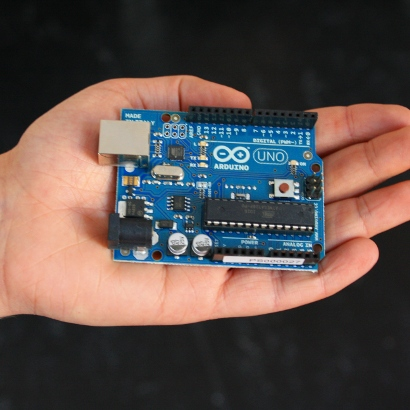
\includegraphics[scale=0.5]{img/arduino/arduino_uno_test.jpg}
     \caption{Arduino}
     \label{Arduino}
\end{figure}

Arduino can sense the environment by receiving input from a variety of sensors and can affect its surroundings by controlling lights, motors, and other actuators. The microcontroller on the board is programmed using the Arduino programming language (based on Wiring) and the Arduino development environment (based on Processing). Arduino projects can be stand-alone or they can communicate with software on running on a computer (e.g. Flash, Processing, MaxMSP).

The boards can be built by hand or purchased preassembled; the software can be downloaded for free. The hardware reference designs (CAD files) are available under an open-source license, you are free to adapt them to your needs.

Arduino received an Honorary Mention in the Digital Communities section of the 2006 Ars Electronica Prix. The Arduino team is: Massimo Banzi, David Cuartielles, Tom Igoe, Gianluca Martino, and David Mellis. Credits


\section{Programação para micro controladores}

\section{Arduino}

% WIKIPEDIA

Arduino is an open-source electronics prototyping platform, designed to make the process of using electronics in multidisciplinary projects more accessible. The hardware consists of a simple open hardware design for the Arduino board with an Atmel AVR processor and on-board I/O support. The software consists of a standard programming language and the boot loader that runs on the board.

Arduino hardware is programmed using a Wiring-based language (syntax + libraries), similar to C++ with some simplifications and modifications, and a Processing-based IDE.[1]

Currently shipping versions can be purchased pre-assembled; hardware design information is available for those who would like to assemble an Arduino by hand. Additionally, variations of the Italian-made Arduino—with varying levels of compatibility—have been released by third parties.

The Arduino project received an honorary mention in the Digital Communities category at the 2006 Prix Ars Electronica.[2][3]

The project began in Ivrea, Italy in 2005 to make a device for controlling student-built interaction design projects less expensively than other prototyping systems available at the time. As of February 2010 more than 120,000 Arduino boards had been shipped.[4] Founders Massimo Banzi and David Cuartielles named the project after a local bar named Arduino.[5] The name is an Italian masculine first name, meaning "strong friend". The English pronunciation is "Hardwin", a namesake of Arduino of Ivrea

\section{Platform}

\subsection{Hardware}

An official Arduino Duemilanove (rev 2009b).

An Arduino board consists of an 8-bit Atmel AVR microcontroller with complementary components to facilitate programming and incorporation into other circuits. An important aspect of the Arduino is the standard way that connectors are exposed, allowing the CPU board to be connected to a variety of interchangeable add-on modules (known as shields). Official Arduinos have used the megaAVR series of chips, specifically the ATmega8, ATmega168, ATmega328, and ATmega1280. A handful of other processors have been used by Arduino compatibles. Most boards include a 5 volt linear regulator and a 16 MHz crystal oscillator (or ceramic resonator in some variants), although some designs such as the LilyPad run at 8 MHz and dispense with the onboard voltage regulator due to specific form-factor restrictions. An Arduino's microcontroller is also pre-programmed with a bootloader that simplifies uploading of programs to the on-chip flash memory, compared with other devices that typically need an external chip programmer.

At a conceptual level, when using the Arduino software stack, all boards are programmed over an RS-232 serial connection, but the way this is implemented varies by hardware version. Serial Arduino boards contain a simple inverter circuit to convert between RS-232-level and TTL-level signals. Current Arduino boards are programmed via USB, implemented using USB-to-serial adapter chips such as the FTDI FT232. Some variants, such as the Arduino Mini and the unofficial Boarduino, use a detachable USB-to-serial adapter board or cable, Bluetooth or other methods. (When used with traditional microcontroller tools instead of the Arduino IDE, standard AVR ISP programming is used.)

The Arduino board exposes most of the microcontroller's I/O pins for use by other circuits. The Diecimila, now superseded by the Duemilanove, for example, provides 14 digital I/O pins, six of which can produce PWM signals, and six analog inputs. These pins are on the top of the board, via female 0.1 inch headers. Several plug-in application "shields" are also commercially available.

The Arduino Nano, and Arduino-compatible Bare Bones Board and Boarduino boards provide male header pins on the underside of the board to be plugged into solderless breadboards.

Sortable table
Arduino	Processor	Flash
KiB	EEPROM
KiB	SRAM
KiB	Digital I/O
pins	...with
PWM	Analog input
pins	Dimensions
Diecimila	ATmega168	16	0.5	1	14	6	6	2.7"x2.1"
Duemilanove	ATmega328	32	1	2	14	6	6	2.7"x2.1"
Uno	ATmega328	32	1	2	14	6	6	2.7"x2.1"
Mega	ATmega1280	128	4	8	54	14	16	4"x2.1"
Fio	ATmega328P	32	1	2	14	6	8	1.1"x1.6"
Mega2560	ATmega2560	256	4	8	54	14	16	4"x2.1"

\subsection{Software}

The Arduino IDE is a cross-platform application written in Java, and is derived from the IDE for the Processing programming language and the Wiring project. It is designed to introduce programming to artists and other newcomers unfamiliar with software development. It includes a code editor with features such as syntax highlighting, brace matching, and automatic indentation, and is also capable of compiling and uploading programs to the board with a single click. There is typically no need to edit makefiles or run programs on the command line.

The Arduino IDE comes with a C/C++ library called "Wiring" (from the project of the same name), which makes many common input/output operations much easier. Arduino programs are written in C/C++, although users only need define two functions to make a runnable program:

setup() – a function run once at the start of a program that can initialize settings

loop() – a function called repeatedly until the board powers off

A typical first program for a microcontroller simply blinks a LED (light-emitting diode) on and off. In the Arduino environment, the user might write a program like this:

\begin{verbatim}
#define LED_PIN 13
 
void setup () {
    pinMode (LED_PIN, OUTPUT);     // enable pin 13 for digital output
}
 
void loop () {
    digitalWrite (LED_PIN, HIGH);  // turn on the LED
    delay (1000);                  // wait one second (1000 milliseconds)
    digitalWrite (LED_PIN, LOW);   // turn off the LED
    delay (1000);                  // wait one second
}
\end{verbatim}

[7]
The above code would not be seen by a standard C++ compiler as a valid program, so when the user clicks the "Upload to I/O board" button in the IDE, a copy of the code is written to a temporary file with an extra include header at the top and a very simple main() function at the bottom, to make it a valid C++ program.
The Arduino IDE uses the GNU toolchain and AVR Libc to compile programs, and uses avrdude to upload programs to the board.
Official hardware

The Arduino Mega2560, uses a surface-mounted ATmega2560, bringing the total memory to 256 kB. It also incorporates the new ATmega8U2 USB chipset.

\subsection{Open hardware and open source}

\subsection{Main article: Open source hardware}

The Arduino hardware reference designs are distributed under a Creative Commons Attribution Share-Alike 2.5 license and are available on the Arduino Web site. Layout and production files for some versions of the Arduino hardware are also available. The source code for the IDE and the on-board library are available and released under the GPLv2 license.[1]

\subsection{Accessory hardware}


\subsection{A prototyping shield, mounted on an Arduino}

Arduino and Arduino-compatible boards make use of shields, which are printed circuit boards that sit atop an Arduino, and plug into the normally supplied pin-headers. These are expansions to the base Arduino. There are many functions of shields, from motor controls, to breadboarding (prototyping).[1]

For example:

\begin{itemize}
\item Arduino Ethernet Shield
\item XBee Shield
\item TouchShield from Liquidware
\item Datalog Shield: RTC, SD card storage, temperature sensing, etc. From NuElectronics
\item USB Host Shield from Circuits@Home
\item Cosmo WiFi Connect from JT5
\item A list of Arduino-compatible shields is maintained at the Arduino Shield List website.
\end{itemize}


